% % % % % % % % % % % % % % % % % % % % % % % % % % % % % % % % % % % % % % % %
% IEEE Style - Double columns, 11pt font, letterpaper
\documentclass[journal, twocolumn, final,11pt,letterpaper]{IEEEtran}	

% Include Latex Packages
\usepackage{etex}	% This package enables the use of many packages

% % Page styles
\usepackage{setspace}	% line spacing package
\doublespacing			% use double spacing
%\linespread{1.6}		% Use linespread to fine tune line spacing, not recommended


% % Figures
\usepackage{float}		% improves interface for floating objects
\usepackage{subfig}		% enables subfloat
\usepackage{graphicx}	% more image type support
\usepackage{circuitikz}
\usepackage{epstopdf}	% automatically convert included eps files to pdf
\usepackage{tikz}
%\usepackage{listings}
\usepackage{color}
\definecolor{dkgreen}{rgb}{0,0.6,0}
\definecolor{gray}{rgb}{0.5,0.5,0.5}
\definecolor{mauve}{rgb}{0.58,0,0.82}

\lstset{frame=tb,
	language=Verilog,
	aboveskip=3mm,
	belowskip=3mm,
	showstringspaces=false,
	columns=flexible,
	basicstyle={\small\ttfamily},
	numbers=none,
	numberstyle=\tiny\color{gray},
	keywordstyle=\color{blue},
	commentstyle=\color{dkgreen},
	stringstyle=\color{mauve},
	breaklines=true,
	breakatwhitespace=true,
	tabsize=3
}
\usetikzlibrary{matrix,calc}
\usetikzlibrary{shapes}

\newcommand*{\circled}[2][red]{
	\tikz[baseline=(char.base)]{
		\node[shape=ellipse,inner sep=1pt,
		draw=#1,
		] (char) {#2};}
}

%isolated term
%#1 - Optional. Space between node and grouping line. Default=0
%#2 - node
%#3 - filling color
\newcommand{\implicantsol}[3][0]{
	\draw[rounded corners=3pt, fill=#3, opacity=0.3] ($(#2.north west)+(135:#1)$) rectangle ($(#2.south east)+(-45:#1)$);
}


%internal group
%#1 - Optional. Space between node and grouping line. Default=0
%#2 - top left node
%#3 - bottom right node
%#4 - filling color
\newcommand{\implicant}[4][0]{
	\draw[rounded corners=3pt, fill=#4, opacity=0.3] ($(#2.north west)+(135:#1)$) rectangle ($(#3.south east)+(-45:#1)$);
}

%group lateral borders
%#1 - Optional. Space between node and grouping line. Default=0
%#2 - top left node
%#3 - bottom right node
%#4 - filling color
\newcommand{\implicantcostats}[4][0]{
	\draw[rounded corners=3pt, fill=#4, opacity=0.3] ($(rf.east |- #2.north)+(90:#1)$)-| ($(#2.east)+(0:#1)$) |- ($(rf.east |- #3.south)+(-90:#1)$);
	\draw[rounded corners=3pt, fill=#4, opacity=0.3] ($(cf.west |- #2.north)+(90:#1)$) -| ($(#3.west)+(180:#1)$) |- ($(cf.west |- #3.south)+(-90:#1)$);
}

%group top-bottom borders
%#1 - Optional. Space between node and grouping line. Default=0
%#2 - top left node
%#3 - bottom right node
%#4 - filling color
\newcommand{\implicantdaltbaix}[4][0]{
	\draw[rounded corners=3pt, fill=#4, opacity=0.3] ($(cf.south -| #2.west)+(180:#1)$) |- ($(#2.south)+(-90:#1)$) -| ($(cf.south -| #3.east)+(0:#1)$);
	\draw[rounded corners=3pt, fill=#4, opacity=0.3] ($(rf.north -| #2.west)+(180:#1)$) |- ($(#3.north)+(90:#1)$) -| ($(rf.north -| #3.east)+(0:#1)$);
}

%group corners
%#1 - Optional. Space between node and grouping line. Default=0
%#2 - filling color
\newcommand{\implicantcantons}[2][0]{
	\draw[rounded corners=3pt, opacity=.3] ($(rf.east |- 0.south)+(-90:#1)$) -| ($(0.east |- cf.south)+(0:#1)$);
	\draw[rounded corners=3pt, opacity=.3] ($(rf.east |- 8.north)+(90:#1)$) -| ($(8.east |- rf.north)+(0:#1)$);
	\draw[rounded corners=3pt, opacity=.3] ($(cf.west |- 2.south)+(-90:#1)$) -| ($(2.west |- cf.south)+(180:#1)$);
	\draw[rounded corners=3pt, opacity=.3] ($(cf.west |- 10.north)+(90:#1)$) -| ($(10.west |- rf.north)+(180:#1)$);
	\fill[rounded corners=3pt, fill=#2, opacity=.3] ($(rf.east |- 0.south)+(-90:#1)$) -|  ($(0.east |- cf.south)+(0:#1)$) [sharp corners] ($(rf.east |- 0.south)+(-90:#1)$) |-  ($(0.east |- cf.south)+(0:#1)$) ;
	\fill[rounded corners=3pt, fill=#2, opacity=.3] ($(rf.east |- 8.north)+(90:#1)$) -| ($(8.east |- rf.north)+(0:#1)$) [sharp corners] ($(rf.east |- 8.north)+(90:#1)$) |- ($(8.east |- rf.north)+(0:#1)$) ;
	\fill[rounded corners=3pt, fill=#2, opacity=.3] ($(cf.west |- 2.south)+(-90:#1)$) -| ($(2.west |- cf.south)+(180:#1)$) [sharp corners]($(cf.west |- 2.south)+(-90:#1)$) |- ($(2.west |- cf.south)+(180:#1)$) ;
	\fill[rounded corners=3pt, fill=#2, opacity=.3] ($(cf.west |- 10.north)+(90:#1)$) -| ($(10.west |- rf.north)+(180:#1)$) [sharp corners] ($(cf.west |- 10.north)+(90:#1)$) |- ($(10.west |- rf.north)+(180:#1)$) ;
}

%Empty Karnaugh map 4x4
\newenvironment{Karnaugh}%
{
	\begin{tikzpicture}[baseline=(current bounding box.north),scale=0.8]
	\draw (0,0) grid (4,4);
	\draw (0,4) -- node [pos=0.9,above right,anchor=south west] {C1C0} node [pos=0.9,below left,anchor=north east] {EQ} ++(135:1);
	%
	\matrix (mapa) [matrix of nodes,
	column sep={0.8cm,between origins},
	row sep={0.8cm,between origins},
	every node/.style={minimum size=0.3mm},
	anchor=8.center,
	ampersand replacement=\&] at (0.5,0.5)
	{
		\& |(c00)| 00         \& |(c01)| 01         \& |(c11)| 11         \& |(c10)| 10         \& |(cf)| \phantom{00} \\
		|(r00)| 00             \& |(0)|  \phantom{0} \& |(1)|  \phantom{0} \& |(3)|  \phantom{0} \& |(2)|  \phantom{0} \&                     \\
		|(r01)| 01             \& |(4)|  \phantom{0} \& |(5)|  \phantom{0} \& |(7)|  \phantom{0} \& |(6)|  \phantom{0} \&                     \\
		|(r11)| 11             \& |(12)| \phantom{0} \& |(13)| \phantom{0} \& |(15)| \phantom{0} \& |(14)| \phantom{0} \&                     \\
		|(r10)| 10             \& |(8)|  \phantom{0} \& |(9)|  \phantom{0} \& |(11)| \phantom{0} \& |(10)| \phantom{0} \&                     \\
		|(rf) | \phantom{00}   \&                    \&                    \&                    \&                    \&                     \\
	};
}%
{
	\end{tikzpicture}
}

%Empty Karnaugh map 2x4
\newenvironment{Karnaughvuit}%
{
	\begin{tikzpicture}[baseline=(current bounding box.north),scale=0.8]
	\draw (0,0) grid (4,2);
	\draw (0,2) -- node [pos=0.7,above right,anchor=south west] {LA/LB} node [pos=0.6,below left,anchor=north east] {S} ++(120:1);
	%
	\matrix (mapa) [matrix of nodes,
	column sep={0.8cm,between origins},
	row sep={0.8cm,between origins},
	every node/.style={minimum size=0.3mm},
	anchor=4.center,
	ampersand replacement=\&] at (0.5,0.5)
	{
		\& |(c00)| 00         \& |(c01)| 01         \& |(c11)| 11         \& |(c10)| 10         \& |(cf)| \phantom{00} \\
		|(r00)| 0             \& |(0)|  \phantom{0} \& |(1)|  \phantom{0} \& |(3)|  \phantom{0} \& |(2)|  \phantom{0} \&                     \\
		|(r01)| 1             \& |(4)|  \phantom{0} \& |(5)|  \phantom{0} \& |(7)|  \phantom{0} \& |(6)|  \phantom{0} \&                     \\
		|(rf) | \phantom{00}  \&                    \&                    \&                    \&                    \&                     \\
	};
}%
{
	\end{tikzpicture}
}

%Empty Karnaugh map 2x2
\newenvironment{Karnaughquatre}%
{
	\begin{tikzpicture}[baseline=(current bounding box.north),scale=0.8]
	\draw (0,0) grid (2,2);
	\draw (0,2) -- node [pos=0.7,above right,anchor=south west] {b} node [pos=0.7,below left,anchor=north east] {a} ++(135:1);
	%
	\matrix (mapa) [matrix of nodes,
	column sep={0.8cm,between origins},
	row sep={0.8cm,between origins},
	every node/.style={minimum size=0.3mm},
	anchor=2.center,
	ampersand replacement=\&] at (0.5,0.5)
	{
		\& |(c00)| 0          \& |(c01)| 1  \\
		|(r00)| 0 \& |(0)|  \phantom{0} \& |(1)|  \phantom{0} \\
		|(r01)| 1 \& |(2)|  \phantom{0} \& |(3)|  \phantom{0} \\
	};
}%
{
	\end{tikzpicture}
}

%Defines 8 or 16 values (0,1,X)
\newcommand{\contingut}[1]{%
	\foreach \x [count=\xi from 0]  in {#1}
	\path (\xi) node {\x};
}

%Places 1 in listed positions
\newcommand{\minterms}[1]{%
	\foreach \x in {#1}
	\path (\x) node {1};
}

%Places 0 in listed positions
\newcommand{\maxterms}[1]{%
	\foreach \x in {#1}
	\path (\x) node {0};
}

%Places X in listed positions
\newcommand{\indeterminats}[1]{%
	\foreach \x in {#1}
	\path (\x) node {X};
}



% % Maths
\usepackage[cmex10]{amsmath}	% Maths
\usepackage{amsfonts,amssymb} 	% maths symbols

% % Tables
\usepackage{booktabs}  % professional-looking tables
\usepackage{multicol} %used for getting multicolumn without page-break
\usepackage{multirow}	% multi-row tables
\usepackage{array}		% define column format of a table

% % Others
\usepackage{caption}	%Customising captions in floating environments
%\usepackage{abstract}
\usepackage{cite}		% cite multiple
\usepackage{fixltx2e}	%added by pilawa, preventing figure* to get ahead of regular figures.
\usepackage{url}		% url display

% %
\hyphenation{op-tical net-works semi-conduc-tor}	% correct bad hyphenation here
\providecommand{\e}[1]{\ensuremath{\times 10^{#1}}}		% use use \e{2} for scientific number expression


% % Optional packages that might be useful
%\usepackage{epsf}		% eps fix
%\usepackage{verbatim}	% verbatim text are not interpreted by the compiler 
%\numberwithin{equation}{section}	% number equation according to section
%\usepackage{xfrac}		% slanted fraction
%\usepackage{pgfplots}	% plot graph
%\usepackage{tikz,pgfplots} % plot graph
%\usepackage{endnotes}	% endnotes


% Title of Document
\title{ECE385 Experiment \#8
	}
\author{
\IEEEauthorblockN{Eric Meyers, Ryan Helsdingen}\\
\IEEEauthorblockA{Section ABG; TAs: Ben Delay, Shuo Liu \\
March 30th, 2016 \\
emeyer7, helsdin2}}
% % % % % % % % % % % % % % % % % % % % % % % % % % % % % % % % % % % % % % % 
\begin{document}
	
%SECTION : Formatting and Title
\maketitle
\singlespacing

%SECTION 1 - Introduction - Eric
\section{Introduction}
The purpose of this lab is to introduce concepts pertaining to USB protocol/communication and VGA display. The main goal of this lab was to connect a USB keyboard to the Altera FPGA and allow a user to control a ball displayed on a VGA-connected monitor. \\

Throughout this lab we interface with both a keyboard through an on-board USB input port and a monitor through a VGA output port on the DE2 board.  Direction keys (W-A-S-D) are used to control the direction of a ball moving on the VGA monitor.  W is up, S is down, A is left, and D is right.  If the ball hits the edge of the screen with no other keys being pushed, it switches direction by 180 degrees.  The ball continues to move in the current direction if no new key is pressed and no screen edge is hit.  The last pressed 8 bit hex scan code is displayed on two of the hex displays and the direction key pushed is shown via the green LEDs on the board.

%SECTION 2 - Description of Circuit / Inputs and Outputs - 
\section{Description of Circuit}
Much of the code needed for the lab was provided.  This included most of the modules used, the framework of the SystemVerilog code needed to connect these modules, and the base C code to make the ball move in two directions on a VGA screen. \\

Tasks that needed to be completed included creating a proper Qsys setup for the NIOS II processor to interface with the CY7C67200, building a top level entity in System Verilog to bring all the files provided together, defining a hardware I/O wrapper to connect the PIO's from the NIOS II to the HPI registers on the CY7C67200 chip, correctly interpreting and implementing the IO\_read and IO\_write methods for accessing the register bank of the CYC67200 chip, using these read and write commands to build USBRead and USBWrite methods, and lastly editing the C code for the ball to function as stated above adding 2 more directions and if/else conditions for boundary cases. 

\subsection{NIOS II System}
The NIOS II System is the processor used for low-speed low-performance tasks such as executing the high level C code.  The NIOS II System is made up of several submodules or PIOs including the NIOS II processor which works with the C code , on-chip memory, SDRAM controller for simplifying interfacing with the SDRAM, SDRAM\_PLL  which provides a phase shifted clock for the SDRAM, the JTAG\_UART submodule which allows for debugging through printf and scanf functions. The PIOs help the C code interact with SystemVerilog by providing addresses for the code to send information to and from various hardware. 



\subsection{CYC67200 chip}
The CYC67200 chip manages information sent through the USB port.  It is controlled by a hardware I/O wrapper in System Verilog that connects the HPI registers to the NIOS II processor.  In Qsys, PIO ports are created for keycode, HPI address, HPI chip select, HPI data, HPI read, and HPI write bits.  HPI\_DATA holds the 16 bit data that will be moved between the FPGA and EZ-OTG.  HPI\_ADDRESS is two bits of the address where the data will be read/written to whether it be HPI DATA, HPI MAILBOX, HPI ADDRESS, or HPI STATUS. Fig. \ref{fig:ports} shows the four registers matching up with their respective addresses.   \\

\begin{figure}[h]
	\centering
	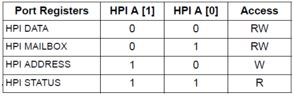
\includegraphics[width=0.45\textwidth]{ports.jpg}
	\caption{Port registers for different addresses. (lab manual)}
	\label{fig:ports}
\end{figure}

The IO\_read and IO\_write methods are used for accessing the register bank of the CYC67200 chip.  We use these read and write commands to build USBRead and USBWrite methods to read and write to the internal memory of the EZ-OTG.

\subsubsection{IO\_read}
To read and return data from the memory location specified by the two bit memory address, we use the IO\_read function. \\

\subsubsection{IO\_write}
To write data to the memory location specified by the two bit memory address, we use the IO\_write function.

Two helper functions, USB\_Read and USB\_Write are used to simplify the process.\\

\subsubsection{USB\_read}
This helper function takes in an address from EZ-OTG memory, writes it to the EZ-OTG address register using IO\_write function, and reads the EZ-OTG data register at that address using IO\_read.  \\

\subsubsection{USB\_write}
This helper function takes in an address from EZ-OTG memory, writes it to the EZ-OTG address register using IO\_write function, and this time writes to the EZ-OTG data register at that address using IO\_write. \\

\textit{Code for Ball Movement}\\
For the ball, C code was added to control ball movement.  Section III of this report labeled 'Purpose of Modules' goes into further detail on each module used in the lab including the ball.sv module.  
  

%SECTION 3 - Purpose of Modules - 
\section{Purpose of Modules}

\subsection{lab8.sv}
This is the top-level module for lab 8.  Inputs include the 50 MHz clock, push button, data and interrupt from the CY7C67200 chip, and data from the SDRAM.  Outputs include the two hex displays, the green LEDs, the DRAM interface, rest of the interface to the CY7C67200, and VGA.  \\

The module includes several instantiations.  hpi\_io\_intf instantiates the interaction between the hardware and usb, nios\_system instantiates the connections for the NIOS II system, vga\_controller, ball, and collor\_mapper instantiate connections for their respective modules.

\subsection{hpi\_io\_intf.sv}
This method takes HPI output values from the NIOS II as input, checks for a call to reset, and if no reset, assigns these values to the proper values to be outputted by the top-level module to the CY7C67200 chip.  Inputs and outputs used are shown below.

\begin{figure}[h]
	\centering
	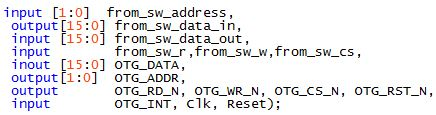
\includegraphics[width=0.45\textwidth]{hpiio.jpg}
	\label{fig:hpiio}
\end{figure}



\subsection{VGA\_controller.sv}
The VGA\_controller manages output to the monitor.  Inputs include clock and reset. Outputs include several sync signals, a pixel clock specified for 25 MHz and 10 bit horizontal and vertical coordinate signals as shown below.

\begin{figure}[h]
	\centering
	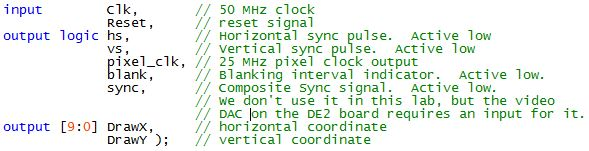
\includegraphics[width=0.45\textwidth]{VGAio.jpg}
	\label{fig:VGAio}
\end{figure}

Most of this module was given to the team.


\subsection{Ball.sv}
This module defines the motion of the ball.  How big the ball size is, how fast and far the steps are for the ball movement, and the x and y coordinate for the ball are all given in this module.  Inputs include the reset, clock, and signals for the four directionals.  Outputs include the 10-bit values for x and y coordinates of the ball as well as size of the ball, BallS.  
  
\begin{figure}[h]
	\centering
	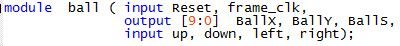
\includegraphics[width=0.45\textwidth]{ballio.jpg}
	\label{fig:ballio}
\end{figure}

Parameters are set to control where the ball can travel and step size of the ball.

\begin{figure}[h]
	\centering
	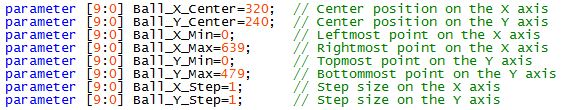
\includegraphics[width=0.45\textwidth]{ballparam.jpg}
	\label{fig:ballparam}
\end{figure}

The following code sets the ball to reverse direction when the ball hits one of its boundaries. \\

\begin{figure}[h]
	\centering
	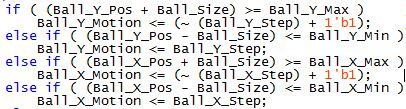
\includegraphics[width=0.45\textwidth]{ballboundary.jpg}
	\label{fig:ballboundary}
\end{figure}

The ball is then given set directions for given key codes from the keyboard as shown below.  Directions are based off directional input values.\\

\begin{figure}[h]
	\centering
	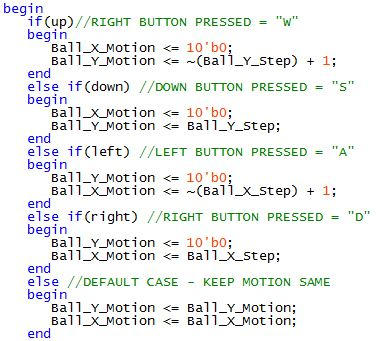
\includegraphics[width=0.45\textwidth]{ballkey.jpg}
	\label{fig:ballkey}
\end{figure}


\subsection{color\_mapper.sv}
The color\_mapper module controls the color of the pixels where the ball is located and maintains proper ball shape as the ball moves from location to location.  Inputs for this module include the coordinates to the center of the ball, the draw coordinates, and the size of the ball.  Outputs include the RGB array for that draw coordinate. \\

\begin{figure}[h]
	\centering
	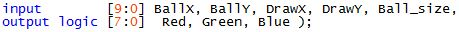
\includegraphics[width=0.45\textwidth]{colorio.jpg}
	\label{fig:colorio}
	\end{figure}

This module was given to the team. \\



%SECTION 4 - Description of USB Protocol & Changes
\section{Description of USB Protocol \& Changes}
The USB protocol in Experiment 8 utilized the Cypress EZ-OTG (CY7C67200) USB controller on board the Altera. The CY7C67200 was used as a host controller and once a USB keyboard is plugged in, the keyboard acts as a device controller.\\

The USB Keyboard is not an interrupt-based device, rather the host must poll the keyboard and send requests to receive the scancode in return. For this, the team must write functions to perform input/output reading and writing. These functions must be used in conjunction with the system verilog hardware that is synthesized to retrieve data and write data. \\

The two functions that were written by the team were in "usb.c" and "io\_handler.c" were pertaining to the reading and writing of data to and from the USB device controller (keyboard).\\

io\_handler.c:
\begin{itemize}
	\item 	void IO\_init(void)
	\item 	void IO\_write(alt\_u8 Address, alt\_u16 Data)
\end{itemize}


\begin{lstlisting}
void IO_write(alt_u8 Address, alt_u16 Data)
{
	*otg_hpi_address = Address;
	*otg_hpi_cs = 0;
	*otg_hpi_w = 0;
	*otg_hpi_data = Data;
	*otg_hpi_w = 1;
	*otg_hpi_cs = 1;
}
\end{lstlisting}
This function takes in parameters as the Address and Data to be written. It then sets the appropriate bits on the signal lines and sends the Data to the otg\_hpi\_data variable to be written to the usb hardware.\\ 

\begin{lstlisting}
alt_u16 IO_read(alt_u8 Address)
{
	alt_u16 temp;
	//printf("%x\n",temp);
	*otg_hpi_address = Address;
	*otg_hpi_cs = 0;
	*otg_hpi_r = 0;
	temp = *otg_hpi_data;
	*otg_hpi_r = 1;
	*otg_hpi_cs = 1;
	return temp;
}
\end{lstlisting}
This function performs similar actions to the IO\_write function in that it must read from a particular address on the USB hardware. The team had to use a temp variable to read it properly, set the appropriate signals, then send the data from otg\_hpi\_data into the temp variable which is then returned to the user by the function.\\

usb.c:
\begin{itemize}
	\item 	void UsbWrite(alt\_u16 Address, alt\_u16 Data)
	\item 	alt\_u16 UsbRead(alt\_u16 Address)
\end{itemize}
\begin{lstlisting}
void UsbWrite(alt_u16 Address, alt_u16 Data)
{
	IO_write(HPI_ADDR, Address);
	IO_write(HPI_DATA, Data);
}
\end{lstlisting}
This function utilizes the two functions written in the previous section (in io\_handler.c) and simply writes the particular address and the data in the parameters.


\begin{lstlisting}
alt_u16 UsbRead(alt_u16 Address)
{
	IO_write(HPI_ADDR, Address);
	alt_u16 temp = IO_read(HPI_DATA);
	return temp;
}
\end{lstlisting}
This function uses the two functions written in io\_handler.c to perform a read on the USB hardware. it first must write the address to HPI\_ADDR to receive the proper address, then the temp variable must store the result of IO\_read from HPI\_Data. 



%SECTION 5 - Schematic/Block Diagram - 
\section{Schematic/Block Diagram}
The Schematic / Block Diagrams for this lab can be found in the Figures section of this document ("Section XI: Figures"). The Top Level Module Diagram can be found in Figure \ref{fig:top-level}, the Ball Module Diagram can be found in Figure \ref{fig:ball}, the VGA Module Diagram can be found in Figure \ref{fig:vga}, and the Color Mapper Module can be found in Figure \ref{fig:color_mapper}.

%SECTION 6 - Post Lab - 
\section{Post Lab}
\begin{table}[htbp]
	\centering
	\begin{tabular}{c|c}	% ccccccc indicates 7 center aligned columns
		\toprule	% top separator
		Resource & Value \\
		\midrule
		LUT & 2663\\
		DSP & 10\\
		Memory (BRAM) & 82,944\\
		Flip-Flop & 646\\
		Frequency &   132.89 MHz\\
		Static Power & 102.09 mW\\
		Dynamic Power &  25.86 mW\\
		Total Power & 203.64 mW\\
		\bottomrule	% bottom separator
	\end{tabular}%	
	\caption{Design Statistics}
	\label{tab:design}
\end{table}

1. What is the difference between VGA\_clk and Clk? \\

\textit{Answer:}The VGA Clock runs at 25MHz to change how wide the individual pixels are, whereas the Clk onboard the processor runs at 50MHz (and does not affect the pixel size).\\

2. In the file io\_handler.h, why is it that the otg\_hpi\_address is defined as an integer pointer while the otg\_hpi\_r is defined as a char pointer? \\

\textit{Answer:} otg\_hpi\_r is a single bit and does not need to be declared as an int (16 bits - it would be a waste of space), whereas otg\_hpi\_address is multiple bits wide and must have multiple bits available to use.\\

3.What are the advantages and/or disadvantages of using a USB interface over PS/2 interface to connect to the keyboard? List any two. \\

\textit{Answer:} PS/2 keyboards aren't polled, but are completely interrupt based. This allows the processor to complete tasks while waiting. Drivers for PS/2 are much simpler than USB keyboard drivers. Another disadvantage is that the USB keyboard only takes in 6 keys every message, so this is limited compared to the PS/2. These are two disadvantages for using a USB keyboard over PS/2.\\

4.  Note that Ball\_Y\_Motion in the above statement may have been changed at the same clock edge that is causing the assignment of Ball\_Y\_pos.  Will the new value of Ball\_Y\_Motion be used, or the old?  How will this impact behavior of the ball during a bounce, and how might that interact with a response to a keypress?  Can you fix it?\\

\textit{Answer:} The new value of Ball\_Y\_Motion that would be used would be the old one and this would make it so that the ball bounces one clock cycle after the keypress is handled. A fix would be to put the assignment inside of the section of code that bounces the ball so that there is no delay in processing. \\

%SECTION 7 - Conclusion
\section{Conclusion}
For experiment 8, the team was successfully able to complete all of the tasks.  The only issue came about in properly writing the C code to interface with the USB drivers. Setting the proper ports in each read/write method was causing errors if done incorrectly. A significant amount of time was spent debugging this interface code.  \\

This lab will prove very important for the final design project, especially if the project involves interfacing with a keyboard input and monitor output.  


\clearpage
\onecolumn
%SECTION 11: Figures
\section{Figures}

\begin{figure} [H]
	\centering
	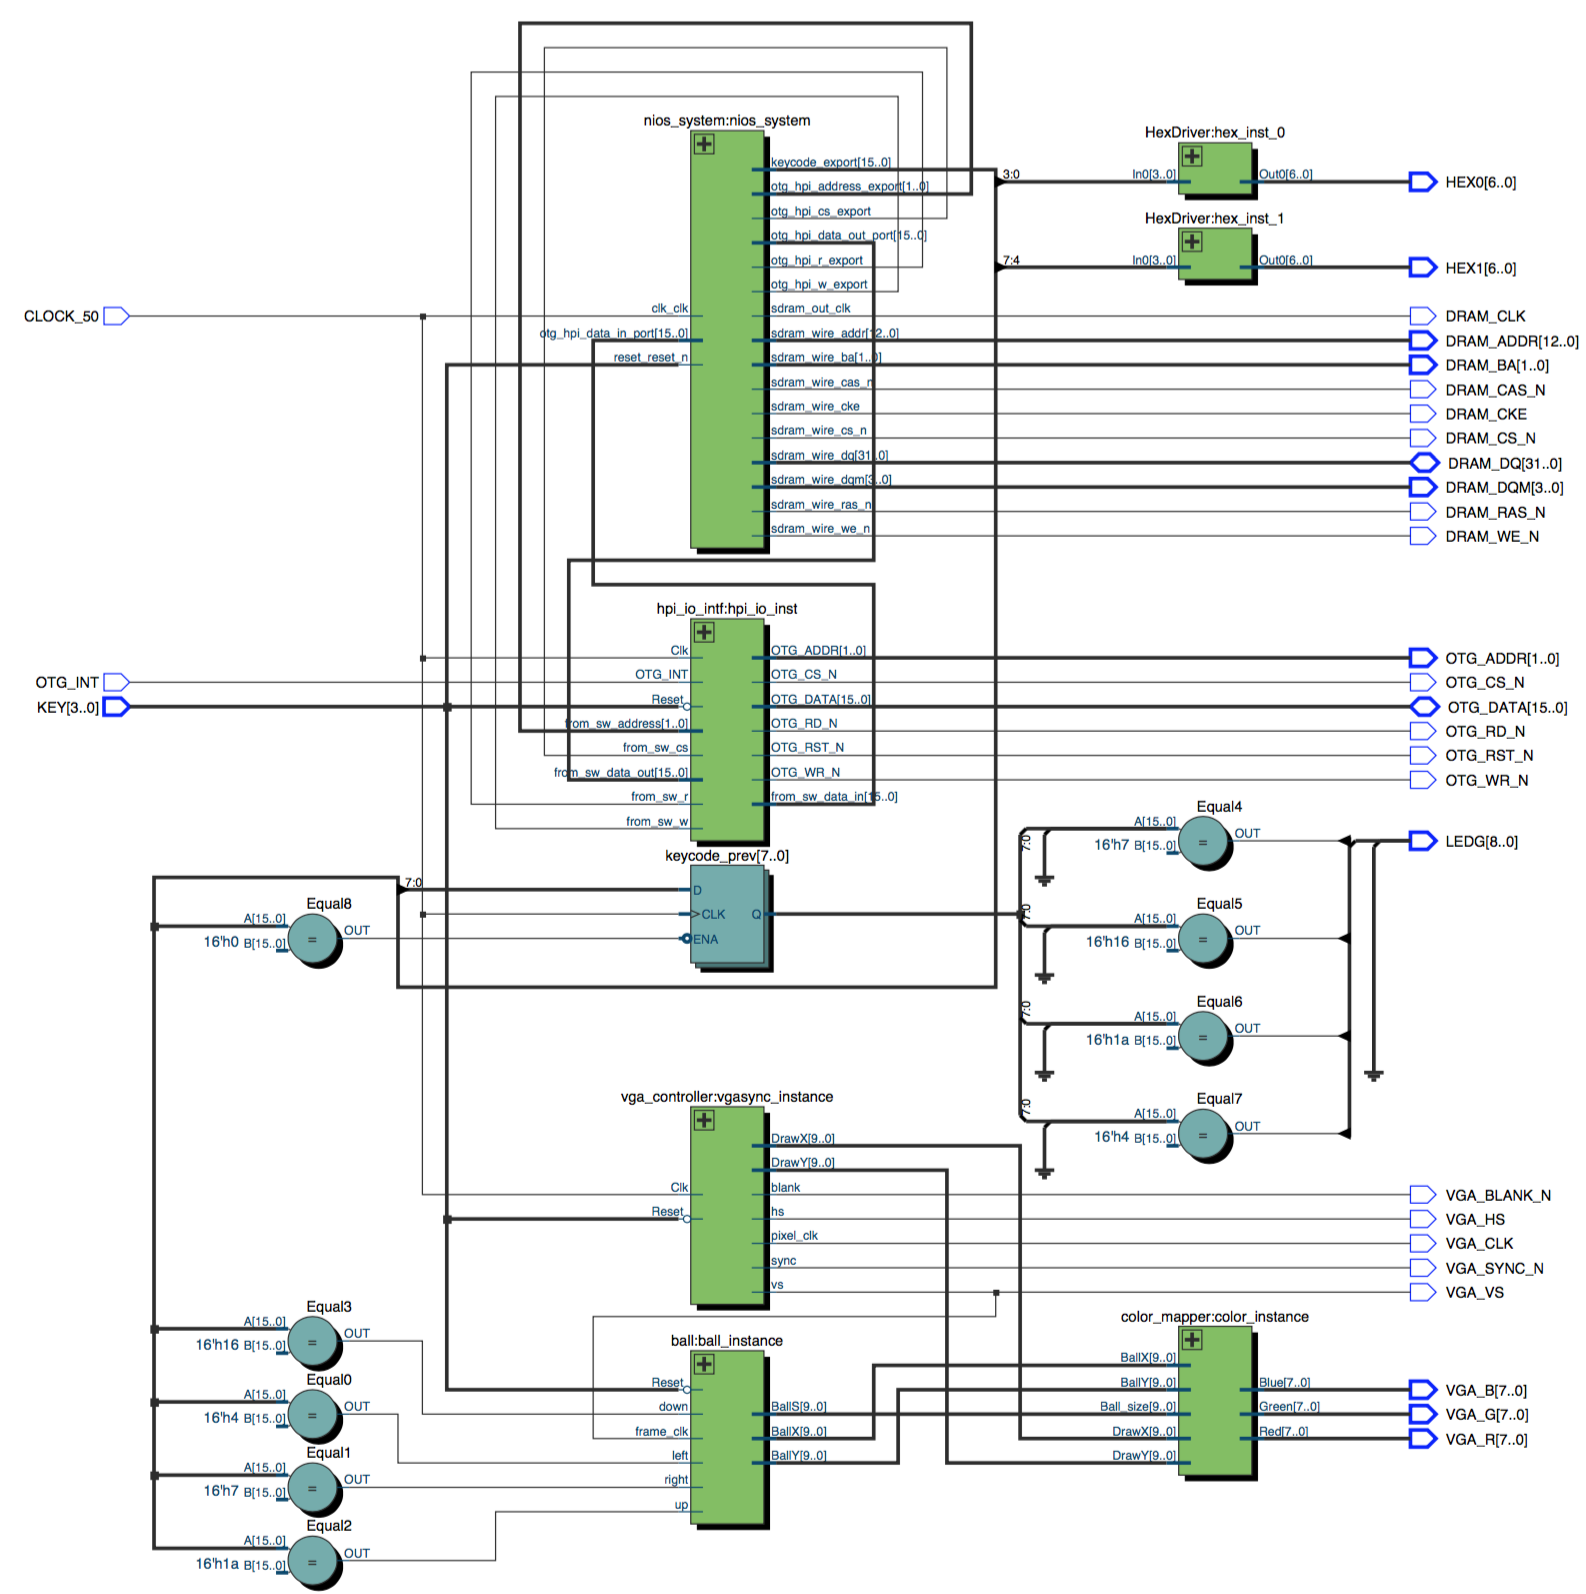
\includegraphics[scale=.5]{top_level_diagram.png}
	\caption{Lab 8 Top Level SV\label{fig:top-level}}
\end{figure}

\begin{figure} [H]
	\centering
	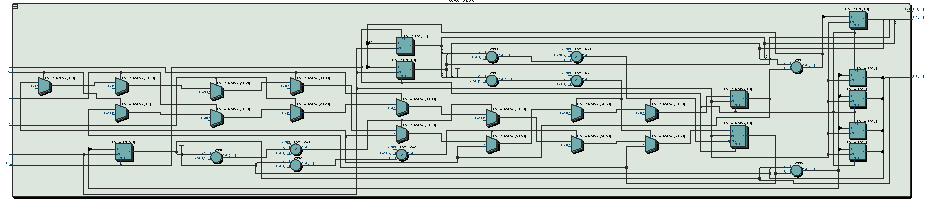
\includegraphics[scale=1]{ball_diagram.pdf}
	\caption{Ball Circuit Diagram\label{fig:ball}}
\end{figure}

\begin{figure} [H]
	\centering
	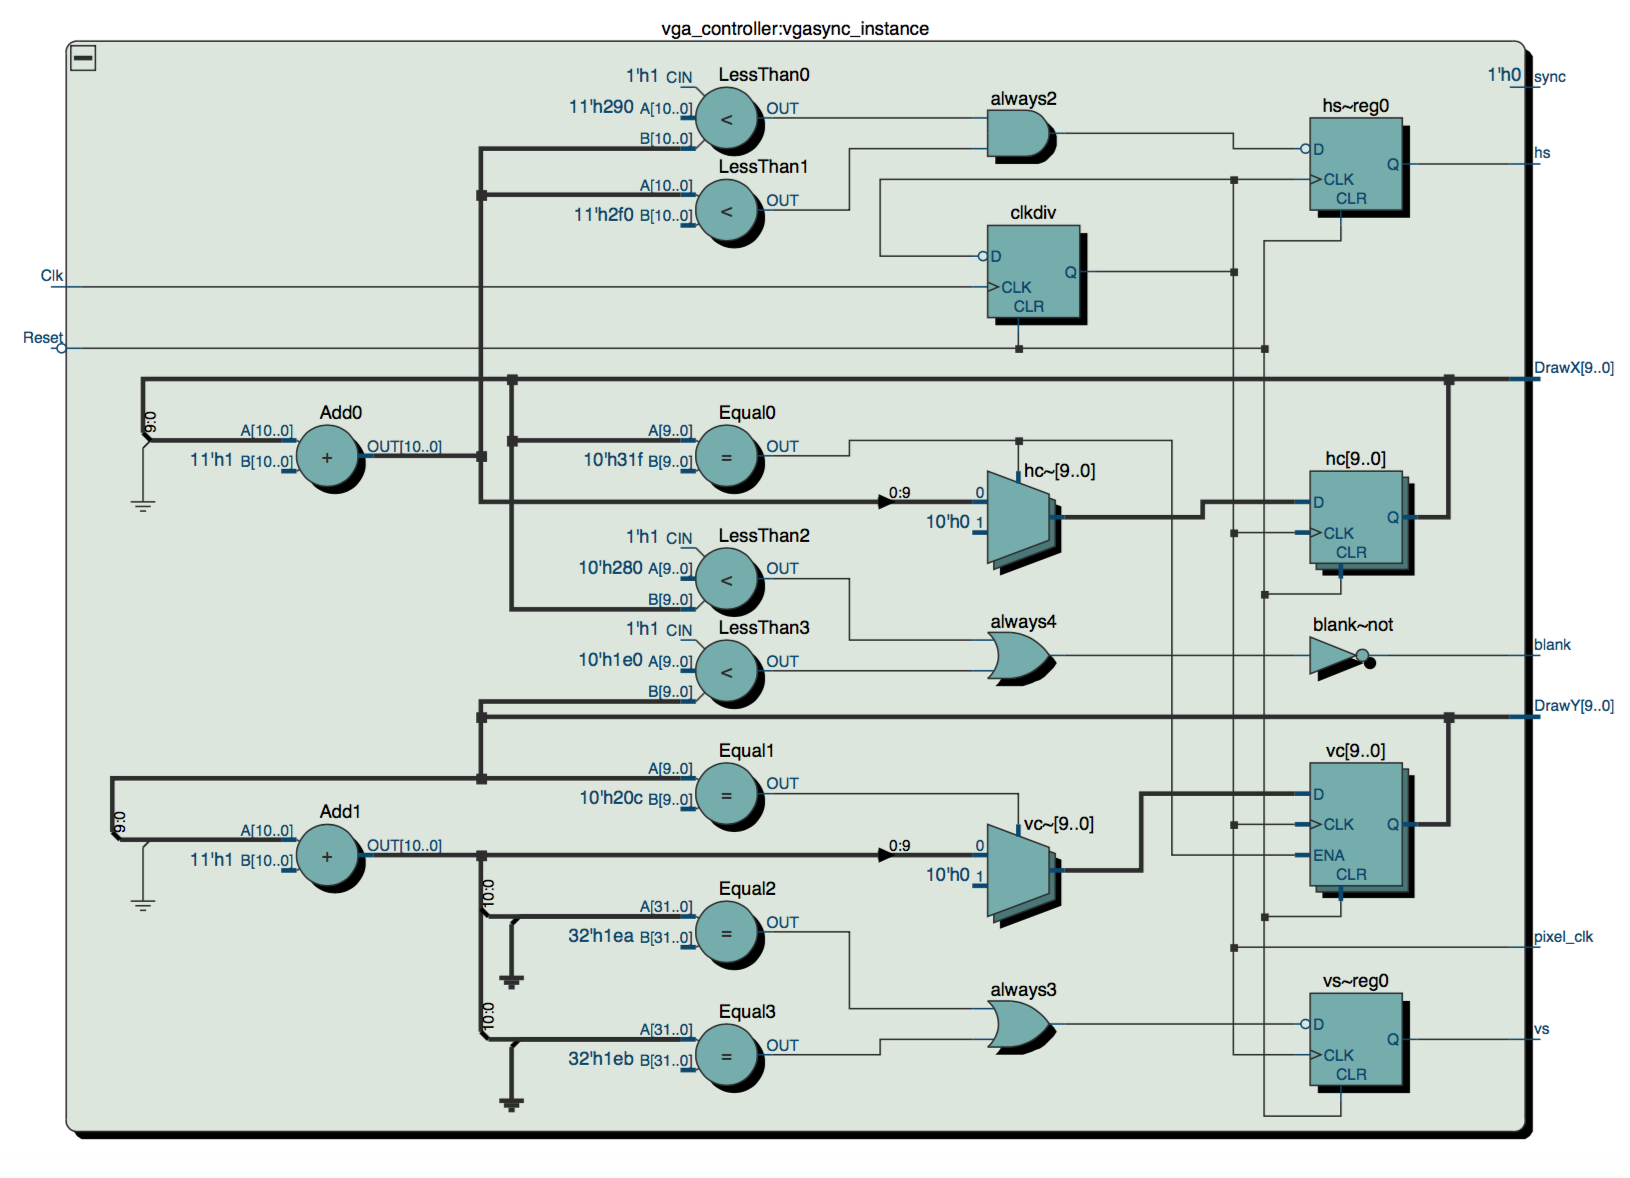
\includegraphics[scale=.5]{vga_diagram.png}
	\caption{VGA Circuit Diagram\label{fig:vga}}
\end{figure}

\begin{figure} [H]
	\centering
	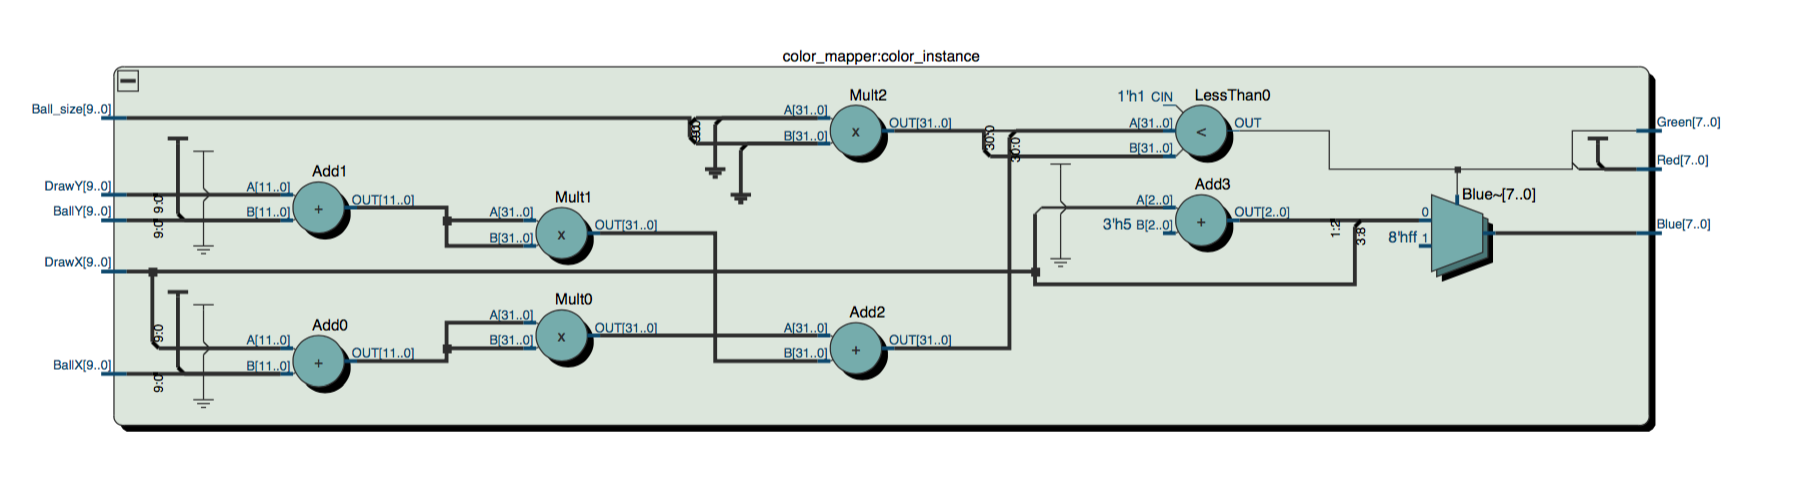
\includegraphics[scale=.5]{color_mapper_diagram.png}
	\caption{Color Mapper Circuit Diagram\label{fig:color_mapper}}
\end{figure}            

     

\section*{Appendix}


\end{document}
